%% Format of the ACM International Conference on AI in Finance (ICAIF): two-column ACM
%% `sigconf`. ICAIF 2026 allowed at most 8 pages, references included, with double-blind
%% review and no supplementary material. Check the call for papers of the target edition.
%%
%% For a double-blind submission, replace the line below with:
%%   \documentclass[sigconf,review,anonymous]{acmart}
\documentclass[sigconf]{acmart}

%% Packages and macros of this paper, loaded after the ACM class.

\usepackage{pgfplots}
\pgfplotsset{compat=1.18}
\usetikzlibrary{arrows.meta,positioning,calc}
\usepackage{needspace}
\usepackage[inline]{enumitem}
\usepackage[capitalize]{cleveref}

% Series colors: one fixed hue per model in every figure (validated for color-vision deficiencies).
\definecolor{cCand}{HTML}{2A78D6}
\definecolor{cRev}{HTML}{EB6834}
\definecolor{cLgb}{HTML}{1BAF7A}
\definecolor{cTfmFt}{HTML}{EDA100}
\definecolor{cTfmZs}{HTML}{E87BA4}
\definecolor{cMom}{HTML}{008300}
\definecolor{cDev}{HTML}{CDE2FB}
\definecolor{cFinal}{HTML}{FBE0D3}

\newcommand{\ric}{Rank~IC}
\newcommand{\etal}{\emph{et~al.}}

% Reads a generated table body inside a tabular: the primitive input is expandable, so a
% row of the file may start with \multicolumn or a rule.
\makeatletter
\def\tablefile#1{\@@input #1 }
\makeatother


%% Rights, DOI and conference information are filled in by ACM after acceptance.
\setcopyright{none}
\settopmatter{printacmref=false}
\renewcommand\footnotetextcopyrightpermission[1]{}

\begin{document}

\title[Do Time-Series Foundation Models Pick Stocks?]{Do Time-Series Foundation Models Pick Stocks? A Leakage-Controlled Evaluation of TimesFM~3 for Daily Cross-Sectional Equity Ranking}

\author{Titouan Salin}
\email{titouan.salin@mail.utoronto.ca}
\affiliation{%
  \institution{University of Toronto}
  \city{Toronto}
  \state{Ontario}
  \country{Canada}}

\begin{abstract}
Time-series foundation models forecast new series without task-specific training, which raises a practical question: can they pick stocks?
We evaluate TimesFM~3 on a realistic task.
Every day it ranks the 100 most liquid U.S.\ stocks by their next five-day return, and a long-only portfolio holds the top 20, net of transaction costs.
The protocol uses point-in-time CRSP, Compustat and I/B/E/S data, an execution lag of one day and purged yearly walk-forward retraining over 2005--2021.
All 70 development trials are recorded for Deflated Sharpe ratios, and a final test on 2022--2025 is run once, with a configuration frozen beforehand.
Zero-shot TimesFM has no ranking skill (\ric{} 0.007), and its forecasts add nothing as features to gradient boosting.
Fine-tuning its last four layers with a cross-sectional correlation loss gives it a significant but modest signal (\ric{} 0.023, information ratio 0.39).
This signal is comparable to LightGBM on market data, but adds nothing to the best model, an equal-weight ensemble of grid-averaged LightGBM with accounting and analyst data and four classic signals (information ratio 0.64).
On the untouched final test, that model earns 6.7\% per year above the equal-weight universe after costs (information ratio 0.60), close to its development estimate but not significant over four years.
\end{abstract}


\ccsdesc[500]{Computing methodologies~Machine learning}
\ccsdesc[300]{Applied computing~Economics}

\keywords{time-series foundation models, TimesFM, stock selection, cross-sectional return prediction, backtest overfitting, transaction costs}

\maketitle
% Page numbers only, without the conference running heads.
\pagestyle{plain}

\section{Introduction}
\label{sec:intro}

Foundation models for time series are pretrained on large collections of series and then forecast new ones zero-shot, often matching models trained on the target data~\cite{das2024timesfm,ansari2024chronos,woo2024moirai,rasul2023lagllama}.
Stock prices are among the most studied series, so a natural question is whether these models can help select stocks.
Forecasting accuracy is the wrong yardstick for that question.
Daily returns are mostly noise; an investor needs a good \emph{ranking} of stocks on each date, and a portfolio built on that ranking must stay profitable after paying for its trades.
At a horizon of a few days, trading costs can erase most of the gross gain~\cite{novymarx2016taxonomy}.

Backtests in this domain are also easy to inflate.
Accounting databases overwrite figures with later restatements, split-adjusted analyst estimates embed splits that had not yet happened~\cite{payne2003ibes}, and filtering surviving stocks hides delisting losses~\cite{shumway1997delisting}.
Even without such leaks, reporting the best of many variants overstates performance~\cite{bailey2014deflated,harvey2016cross}.
A meaningful evaluation of a foundation model must control all of these, and compare it with strong conventional baselines under the same rules.

We ask whether TimesFM~3, zero-shot or fine-tuned, improves the cross-sectional ranking of U.S.\ stocks and the resulting portfolio, compared with simple factor signals and gradient-boosted trees, out of sample and after costs.
Our contributions are:
\begin{itemize}
\item \textbf{A leakage-controlled protocol} for daily cross-sectional ranking (\cref{sec:setup}).
It combines point-in-time accounting and analyst data, delisting returns, a one-day execution lag and purged walk-forward retraining.
A registry of every development trial feeds Deflated Sharpe ratios, and a final test is opened once with a configuration frozen in advance.
\item \textbf{A systematic evaluation of TimesFM~3} (\cref{sec:models,sec:dev}): zero-shot forecasts, forecasts as features, fine-tuning with a cross-sectional correlation loss at two training lengths over five seeds, and ensembles with simple signals.
\item \textbf{Findings that survive an untouched test period} (\cref{sec:final}).
Zero-shot TimesFM has no ranking skill, and fine-tuning gives it a real but modest signal that adds nothing to the best model.
That model combines a grid-averaged LightGBM with accounting and analyst data and four classic signals, and it reproduces its development performance on 2022--2025.
\item \textbf{Practical lessons} (\cref{sec:discussion}): turnover rather than ranking accuracy decides profitability, selecting hyperparameters on a noisy metric costs signal, and an information ratio earned in a single crisis does not carry over.
\end{itemize}

\section{Related Work}
\label{sec:related}

\paragraph{Predictable patterns in returns.}
Stocks that fell over the past week tend to rebound (short-term reversal)~\cite{jegadeesh1990evidence,lehmann1990fads}, and winners of the past year, skipping the last month, tend to keep winning (momentum)~\cite{jegadeesh1993returns,carhart1997persistence}.
Prices drift after earnings surprises~\cite{bernard1989post,livnat2006comparing} and analyst revisions~\cite{chan1996momentum}, and profitability and value carry information~\cite{novymarx2013other,fama2015five}.
Many anomalies weaken once trading costs are charged~\cite{novymarx2016taxonomy}, especially short-horizon ones.

\paragraph{Machine learning for stock selection.}
Gu \etal~\cite{gu2020empirical} show that trees and neural networks improve monthly return prediction from firm characteristics.
Krauss \etal~\cite{krauss2017deep} report large gross profits from daily statistical arbitrage with deep networks and gradient-boosted trees, profits that shrink after costs.
We use LightGBM~\cite{ke2017lightgbm}, trained on ranked features as in~\cite{gu2020empirical}, as the main conventional model.

\paragraph{Time-series foundation models.}
TimesFM~\cite{das2024timesfm} is a decoder-only transformer over patches of a series, building on patch-based models~\cite{nie2023patchtst}; Chronos~\cite{ansari2024chronos}, Moirai~\cite{woo2024moirai} and Lag-Llama~\cite{rasul2023lagllama} pursue the same zero-shot goal.
They are mainly evaluated on forecasting accuracy.
We instead measure the economic value of TimesFM~3~\cite{timesfm3} forecasts for ranking stocks after costs.

\paragraph{Backtest overfitting and data pitfalls.}
The Deflated Sharpe ratio~\cite{bailey2014deflated} corrects a Sharpe ratio for the number of trials, Harvey \etal~\cite{harvey2016cross} call for higher significance thresholds, and purging overlapping labels prevents a subtler leak~\cite{lopezdeprado2018advances}.
Ignoring delisting returns biases returns upward~\cite{shumway1997delisting}, and split-adjusted I/B/E/S data distort ratios to past prices~\cite{payne2003ibes}.

\section{Task, Data and Protocol}
\label{sec:setup}

\paragraph{Prices.}
We use the CRSP daily stock file from January 1995 to December 2025.
The training universe defined below spans 7,550 trading days and 4,011 distinct stocks.
We keep ordinary common shares of U.S.\ companies listed on a U.S.\ exchange, using the share codes known at each date.
In the current CRSP format, a delisting return sits on a separate row that the standard common-stock filter removes; we keep these rows and set a missing delisting return to $-30\%$~\cite{shumway1997delisting}.
Nasdaq volumes are adjusted for double counting~\cite{gao2010marketing}.
Factor returns~\cite{fama2015five,carhart1997persistence} and the S\&P~500 are used only for reporting.

\paragraph{Accounting and analyst data.}
Quarterly accounting data come from the point-in-time Compustat tables, because later revisions replace the figures investors saw at the time.
Even there, the main value column matches the first-reported figure in only 60--70\% of quarters before 2015.
Taking the as-reported column when it is filled, and the main column otherwise, matches the first monthly snapshot in over 99.7\% of quarters from 1998 to 2024.
A quarter becomes usable only after that snapshot, and a late filing delays the quarters after it.
Analyst data use the \emph{unadjusted} I/B/E/S consensus for the current fiscal year, divided by the price on the date of the consensus, because the split-adjusted table rewrites past estimates for later splits~\cite{payne2003ibes}.
A consensus is usable from the day after its statistics date and an earnings surprise from the day after its announcement.
Records expire after 270, 45 and 100 days respectively.

\paragraph{Universes, target and timing.}
Each month-end, using only data known then, we build two universes that apply from the next session.
The \emph{training universe} holds the 1,000 largest stocks by market value with a price of at least \$5 and 252 days of history.
The \emph{tradable universe} holds the 100 stocks with the largest 63-day median dollar volume among the 500 largest.
A signal computed after the close of day $t$ is executed at the close of $t{+}1$, and the target is the return from the close of $t{+}1$ to the close of $t{+}6$, minus its mean over the training universe $U_t$:
\begin{equation}
y_{i,t} = R_{i,t} - \frac{1}{|U_t|}\sum_{j\in U_t} R_{j,t},\qquad R_{i,t} = \prod_{k=2}^{6} (1 + r_{i,t+k}) - 1.
\label{eq:target}
\end{equation}
Models learn the percentile rank of $y_{i,t}$ within each date.

\paragraph{Portfolio and costs.}
The long-only portfolio targets 20 equal-weight stocks, with decisions taken every day.
A holding is sold only when its rank in the tradable universe falls below 40, and the best-ranked stocks replace it.
A position above 7.5\% is cut back to 5\%, and a delisted holding moves to cash.
Every trade pays 2, 5 or 10 basis points (bp) per side, 5\,bp being the central scenario; a \emph{measured} scenario charges each stock's closing quoted half-spread plus 1\,bp.
The benchmark is the equal-weight tradable universe, which earned 10.7\% per year over 2005--2021, like the S\&P~500.

\begin{figure}[t]
\centering
% Evaluation protocol: data periods, one walk-forward fold, and the timing of one decision.
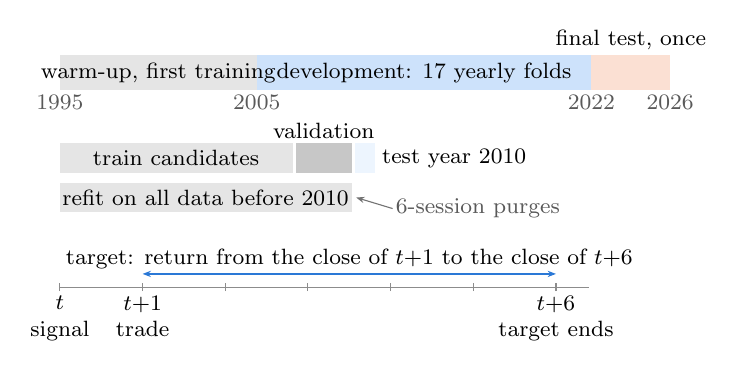
\begin{tikzpicture}[x=0.25cm, y=1cm, font=\footnotesize, every node/.style={inner sep=1pt}]
  % Data periods (x = years since 1995).
  \fill[black!10] (0,0) rectangle (10,0.45);
  \fill[cDev] (10,0) rectangle (27,0.45);
  \fill[cFinal] (27,0) rectangle (31,0.45);
  \node at (5,0.225) {warm-up, first training};
  \node at (18.5,0.225) {development: 17 yearly folds};
  \node[anchor=south] at (29,0.47) {final test, once};
  \foreach \x/\label in {0/1995, 10/2005, 27/2022, 31/2026}
    \node[anchor=north, text=black!65] at (\x,-0.02) {\label};

  % One fold: test year 2010, with purges between phases.
  \begin{scope}[yshift=-1.05cm]
    \fill[black!10] (0,0) rectangle (11.85,0.38);
    \fill[black!22] (12,0) rectangle (14.85,0.38);
    \fill[cDev!100!black!35] (15,0) rectangle (16,0.38);
    \node at (5.9,0.19) {train candidates};
    \node[anchor=south] at (13.4,0.4) {validation};
    \node[anchor=west] at (16.2,0.19) {test year 2010};
    \fill[black!10] (0,-0.5) rectangle (14.85,-0.12);
    \node at (7.4,-0.31) {refit on all data before 2010};
    \draw[black!55, -{Stealth[length=3pt]}] (16.9,-0.45) node[anchor=west, text=black!65] {6-session purges} -- (15.05,-0.31);
  \end{scope}

  % Timing of one decision, on its own scale.
  \begin{scope}[yshift=-2.5cm, x=1.05cm]
    \draw[black!45] (0,0) -- (6.4,0);
    \foreach \k in {0,...,6} \draw[black!45] (\k,-0.05) -- (\k,0.05);
    \node[anchor=north, align=center] at (0,-0.07) {$t$\\signal};
    \node[anchor=north, align=center] at (1,-0.07) {$t{+}1$\\trade};
    \node[anchor=north, align=center] at (6,-0.07) {$t{+}6$\\target ends};
    \draw[cCand, line width=1pt, {Stealth[length=3pt]}-{Stealth[length=3pt]}] (1,0.17) -- (6,0.17);
    \node[anchor=south] at (3.5,0.19) {target: return from the close of $t{+}1$ to the close of $t{+}6$};
  \end{scope}
\end{tikzpicture}

\caption{Evaluation protocol. Top: data periods. Middle: one development fold (test year 2010); hyperparameters are chosen on the three preceding years before a refit on all earlier data, with a 6-session purge between phases. Bottom: timing of one decision.}
\Description{A timeline from 1995 to 2026 with three periods: warm-up and first training from 1995 to 2004, development with 17 yearly folds from 2005 to 2021, and a final test run once from 2022 to 2025. Below, one fold shows training data, three validation years and the test year 2010, separated by purges. At the bottom, a decision timeline shows the signal at day t, the trade at t+1 and the target return from t+1 to t+6.}
\label{fig:protocol}
\end{figure}

\paragraph{Walk-forward protocol.}
Each development year from 2005 to 2021 (17 folds) is predicted by a model trained on all earlier data, with hyperparameters chosen on the three preceding years by validation \ric{} (\cref{fig:protocol}).
The final test, 2022--2025, is refused by the code unless explicitly unlocked, and was run once with a configuration recorded before any of its results were computed.

\paragraph{Metrics and selection rules.}
The \ric{} is the Spearman correlation between scores and targets across tradable stocks, averaged over dates, with Newey--West $t$-statistics (10 lags)~\cite{newey1987simple}.
Paired comparisons use a moving-block bootstrap~\cite{kunsch1989jackknife} of daily differences (21-day blocks, 2,000 draws).
For portfolios we report the annualized net active return, the information ratio (IR), the six-factor alpha and the one-way turnover.
All 70 development runs are registered, and the Deflated Sharpe ratio (DSR)~\cite{bailey2014deflated} uses their number and the variance of their Sharpe ratios.
Rules fixed beforehand: models are compared by net IR at 5\,bp; a more complex model replaces a simpler one only if a bootstrap interval of their \ric{} or return difference excludes zero; and a result is established only if its $t$ exceeds 2 \emph{and} its DSR exceeds 0.95.

\section{Models}
\label{sec:models}

\paragraph{Simple signals.}
Four signals need no fitting: 12--1 momentum~\cite{jegadeesh1993returns}, minus the past five-day return (reversal)~\cite{jegadeesh1990evidence}, the standardized earnings surprise (SUE)~\cite{livnat2006comparing}, and the three-month revision of the consensus forecast scaled by price~\cite{chan1996momentum}.

\begin{table}[t]
\caption{Features. Each value at date $t$ only uses data available at the close of $t$; stock-level variables are replaced by their centred percentile rank within each date over the training universe.}
\label{tab:features}
\footnotesize
\begin{tabular}{@{}p{0.25\linewidth}p{0.71\linewidth}@{}}
\toprule
Group & Variables \\
\midrule
Past returns (11) & log returns over 1, 5, 10, 21, 63, 126 and 252 days; 12--1 momentum; gaps to the 20-, 50- and 200-day moving averages of the log price \\
Risk (8) & drawdown from the 252-day high; volatility over 5, 21 and 63 days; largest daily return over 21 days; 63-day skewness; 252-day market beta; 63-day idiosyncratic volatility \\
Liquidity and size (6) & log 21-day dollar volume; 5- to 63-day volume ratio; 21-day share turnover; 21-day Amihud illiquidity; log market value; log listing age \\
Market (3) & market return over 5 and 21 days; 21-day market volatility (not ranked) \\
Accounting (13) & return on assets and on equity; gross profitability; leverage; cash to assets; current ratio; asset, sales and earnings growth; book-to-market; earnings, sales and EBITDA yields \\
Analysts (7) & consensus EPS to price; its 1- and 3-month revisions; balance of upward and downward revisions; dispersion; log number of analysts; standardized earnings surprise \\
\bottomrule
\end{tabular}
\end{table}

\paragraph{Tabular models.}
The market features are 25 stock-level variables (returns from 1 to 252 days, gaps to moving averages, volatility, beta, idiosyncratic volatility, liquidity and size) and 3 market-level ones.
We add 13 accounting variables (Acc) and 7 analyst variables (Ana), listed in \cref{tab:features}.
Stock-level variables are replaced by their centred percentile rank within each date.
LightGBM~\cite{ke2017lightgbm} (learning rate 0.02, 50\% feature and row subsampling, L2 penalty 10) has a grid of 7 or 31 leaves, 500 or 5,000 minimum samples per leaf and 50 to 400 rounds, and one setting is \emph{selected} each year on validation.
Because the selection changed in almost every year, we also test a \emph{grid average}: the four tree settings are fit on all past data, and the within-date ranks of their predictions after 100, 200 and 400 rounds are averaged (12 models).

\paragraph{TimesFM~3 zero-shot.}
TimesFM~3~\cite{timesfm3} is a decoder-only transformer with 330.7M parameters that reads 32-step input patches and writes 64-step output patches with quantiles from 0.1 to 0.9.
In univariate mode, each forecast reads up to the last 512 daily returns of a stock, with missing days set to zero.
The score is the forecast cumulative return over $t{+}2$ to $t{+}6$; we also test the log price index as input.
The forecast width and asymmetry, added with the score as ranked LightGBM features, are computed over the training universe.
The width tracks the realized volatility of the next five days (rank correlation 0.60), which confirms that the model is fed correctly.

\paragraph{Fine-tuning.}
The package documents only inference and its decoding blocks gradients; calling the undecorated function reproduces the inference outputs exactly.
We train the last four transformer layers and the output head (66.3M parameters).
Each step draws one training date and 64 stocks of the training universe with a full 512-day context.
The score $s_i$ sums the median forecasts over $t{+}2$ to $t{+}6$, and the loss is minus its correlation with the realized sum of returns $y_i$:
\begin{equation}
\mathcal{L} = -\frac{\sum_i (s_i-\bar s)(y_i-\bar y)}{\lVert s-\bar s\rVert\,\lVert y-\bar y\rVert},
\label{eq:loss}
\end{equation}
which rewards the ranking within a date and ignores the market level.
We use AdamW (learning rate $3\times10^{-5}$, weight decay 0.01) with gradient clipping at 1, and skip the steps whose gradient is not finite (about 3\%, from a square root in the model's input normalization).
These settings, with 1,000 steps, were fixed on data before 2005, so no development year was used to tune them.
The model is retrained every three years on all windows labelled before each block, with five seeds whose within-date ranks are averaged.
One follow-up, declared in advance after the development results, changes only the number of steps to 10,000, which takes about 48 minutes per run on one RTX A4500 GPU.

\paragraph{Ensembles.}
Ensembles average the within-date percentile ranks of their members, with equal weights and nothing fitted, and every ensemble was listed before its results were computed.
The \textbf{primary model} gives equal weights to the grid-averaged LightGBM with market, accounting and analyst features (averaged over three seeds) and to the four simple signals.

\section{Development Results (2005--2021)}
\label{sec:dev}

\begin{table*}[t]
\caption{Development results, 2005--2021 (4,275 signal dates, 17 yearly folds). The portfolio holds 20 stocks against the equal-weight tradable universe; returns are net of 5\,bp per side unless stated. The DSR accounts for all 70 registered trials. \emph{Selected}: one LightGBM setting chosen each year; \emph{grid average}: 12 settings averaged without selection.}
\label{tab:dev}
\footnotesize
\setlength{\tabcolsep}{5pt}
\begin{tabular}{@{}lrrrrrrr@{}}
\toprule
Model & \ric{} & $t$ & Net active (\%/yr) & IR & IR at 10\,bp & Turnover (\%/yr) & DSR \\
\midrule
\tablefile{tables/dev_results.tex}
\bottomrule
\end{tabular}
\end{table*}

\begin{table*}[t]
\caption{Paired differences on the development period, with block-bootstrap intervals (21-day blocks, 2,000 draws). Bold intervals exclude zero; they are not corrected for multiple comparisons.}
\label{tab:dev-gaps}
\footnotesize
\begin{tabular}{@{}lll@{}}
\toprule
Comparison (A minus B) & \ric{} difference [95\% CI] & Net return difference, \%/yr [95\% CI] \\
\midrule
\tablefile{tables/dev_gaps.tex}
\bottomrule
\end{tabular}
\end{table*}

\begin{figure}[t]
\centering
% Cumulative net active return, 2005-2025. Data: figures/data/cumulative_active.tsv (export_data.py).
\begin{tikzpicture}
\begin{axis}[
  width=0.93\linewidth, height=5.3cm,
  xmin=2005, xmax=2026, ymin=-60, ymax=180,
  xtick={2005,2009,2013,2017,2021,2025},
  ytick={-50,0,50,100,150},
  x tick label style={/pgf/number format/1000 sep={}},
  tick label style={font=\footnotesize, text=black!75},
  ylabel={Cumulative net active (\%)}, ylabel style={font=\footnotesize},
  ymajorgrids, grid style={black!9},
  axis line style={black!35}, tick style={black!35}, tick align=outside,
  axis x line*=bottom, axis y line*=left,
  legend style={font=\footnotesize, draw=none, fill=none, at={(0.5,-0.14)}, anchor=north, column sep=5pt},
  legend columns=3, legend cell align=left,
]
\fill[black!6] (axis cs:2022,-60) rectangle (axis cs:2026,180);
\node[font=\footnotesize, text=black!60, anchor=north] at (axis cs:2024,178) {final test};
\draw[black!45] (axis cs:2005,0) -- (axis cs:2026,0);
\addplot[cCand, line width=1.2pt] table[x=t, y=candidate, col sep=tab] {figures/data/cumulative_active.tsv};
\addlegendentry{Primary model}
\addplot[cRev, line width=0.9pt, dashed] table[x=t, y=reversal, col sep=tab] {figures/data/cumulative_active.tsv};
\addlegendentry{Reversal}
\addplot[cLgb, line width=0.9pt, dash dot] table[x=t, y=lightgbm, col sep=tab] {figures/data/cumulative_active.tsv};
\addlegendentry{LightGBM}
\addplot[cTfmFt, line width=1.2pt] table[x=t, y=tfmft, col sep=tab] {figures/data/cumulative_active.tsv};
\addlegendentry{TimesFM FT}
\addplot[cTfmZs, line width=0.9pt, densely dotted] table[x=t, y=tfmzs, col sep=tab] {figures/data/cumulative_active.tsv};
\addlegendentry{TimesFM zero-shot}
\end{axis}
\end{tikzpicture}

\caption{Cumulative net active return against the equal-weight tradable universe (sum of daily active returns, 5\,bp per side). The shaded area is the final test, where the portfolios restart from cash. TimesFM FT is the 10k-step fine-tuned model.}
\Description{Line chart of cumulative net active return from 2005 to 2025. The primary model and reversal end near 140 and 130 percent, LightGBM and fine-tuned TimesFM near 80 and 95 percent, and zero-shot TimesFM declines to about minus 40 percent. Reversal gains most of its lead in 2008 to 2010.}
\label{fig:cumulative}
\end{figure}

\begin{figure*}[t]
\centering
% Left: Rank IC by year. Right: net active return against cost. Data from export_data.py.
\pgfplotsset{
  paperaxis/.style={
    tick label style={font=\footnotesize, text=black!75},
    label style={font=\footnotesize},
    ymajorgrids, grid style={black!9},
    axis line style={black!35}, tick style={black!35}, tick align=outside,
    axis x line*=bottom, axis y line*=left,
    legend style={font=\footnotesize, draw=none, fill=white, fill opacity=0.85, text opacity=1},
    legend cell align=left,
  },
}
\begin{tikzpicture}
\begin{axis}[
  paperaxis, name=ic,
  width=0.47\textwidth, height=5.0cm,
  xmin=2004.5, xmax=2025.5, ymin=-0.045, ymax=0.10,
  xtick={2005,2009,2013,2017,2021,2025},
  x tick label style={/pgf/number format/1000 sep={}},
  yticklabel style={/pgf/number format/.cd, fixed, precision=2},
  ylabel={\ric{} (yearly mean)},
  legend style={at={(0.5,1.03)}, anchor=south, fill=none}, legend columns=3,
]
\fill[black!6] (axis cs:2021.5,-0.045) rectangle (axis cs:2025.5,0.10);
\node[font=\footnotesize, text=black!60, anchor=north] at (axis cs:2023.5,0.099) {final test};
\draw[black!45] (axis cs:2004.5,0) -- (axis cs:2025.5,0);
\addplot[cCand, line width=1.1pt, mark=*, mark size=1.5pt] table[x=year, y=candidate, col sep=tab] {figures/data/rank_ic_by_year.tsv};
\addlegendentry{Primary model}
\addplot[cTfmFt, line width=1.1pt, mark=triangle*, mark size=1.9pt] table[x=year, y=tfmft, col sep=tab] {figures/data/rank_ic_by_year.tsv};
\addlegendentry{TimesFM FT 10k}
\addplot[cTfmZs, line width=0.9pt, densely dotted, mark=square*, mark size=1.3pt, mark options={solid}] table[x=year, y=tfmzs, col sep=tab] {figures/data/rank_ic_by_year.tsv};
\addlegendentry{TimesFM zero-shot}
\end{axis}

\begin{axis}[
  paperaxis,
  at={($(ic.east)+(1.2cm,0)$)}, anchor=west,
  width=0.47\textwidth, height=5.0cm,
  xmin=1.5, xmax=10.5, ymin=-11, ymax=11,
  xtick={2,5,10},
  xlabel={Cost per side (bp)}, ylabel={Net active return (\%/yr)},
  ytick={-10,-5,0,5,10},
  legend style={at={(0.02,0.02)}, anchor=south west}, legend columns=2,
]
\draw[black!45] (axis cs:1.5,0) -- (axis cs:10.5,0);
\addplot[cCand, line width=1.1pt, mark=*, mark size=1.5pt] table[x=cost, y=candidate, col sep=tab] {figures/data/cost_sensitivity.tsv};
\addlegendentry{Primary (2,386\%)}
\addplot[cRev, line width=0.9pt, dashed, mark=diamond*, mark size=1.9pt, mark options={solid}] table[x=cost, y=reversal, col sep=tab] {figures/data/cost_sensitivity.tsv};
\addlegendentry{Reversal (4,942\%)}
\addplot[cLgb, line width=0.9pt, dash dot, mark=pentagon*, mark size=1.7pt, mark options={solid}] table[x=cost, y=lightgbm, col sep=tab] {figures/data/cost_sensitivity.tsv};
\addlegendentry{LightGBM (4,347\%)}
\addplot[cTfmFt, line width=1.1pt, mark=triangle*, mark size=1.9pt] table[x=cost, y=tfmft, col sep=tab] {figures/data/cost_sensitivity.tsv};
\addlegendentry{TimesFM FT (3,535\%)}
\addplot[cMom, line width=0.9pt, loosely dashed, mark=square*, mark size=1.3pt, mark options={solid}] table[x=cost, y=momentum, col sep=tab] {figures/data/cost_sensitivity.tsv};
\addlegendentry{Momentum (215\%)}
\end{axis}
\end{tikzpicture}

\caption{Left: yearly \ric{} of the primary model and TimesFM, with the final test shaded. Right: development net active return against the cost per side; the legend gives each model's annual turnover, which sets the slope of each line.}
\Description{Left panel: yearly Rank IC from 2005 to 2025 for the primary model, fine-tuned TimesFM and zero-shot TimesFM; the primary model is positive in most years and zero-shot TimesFM often negative. Right panel: net active return at costs of 2, 5 and 10 basis points per side; reversal falls from about 10 to 2 percent, LightGBM from 6.5 to minus 0.4 percent, the primary model from 8.2 to 4.4 percent, fine-tuned TimesFM from 6.4 to 0.8 percent, and momentum stays near 1 percent.}
\label{fig:ic-cost}
\end{figure*}

\paragraph{Baselines.}
\cref{tab:dev} reports the development results, \cref{tab:dev-gaps} the paired comparisons and \cref{fig:cumulative} the cumulative active returns.
All four simple signals have a positive \ric{} with $t>2$.
Reversal earns the largest net active return of any single model (+6.9\%/yr, IR 0.54), but it trades 49 times its capital a year and earned most of it in 2008--2010 (+26.6\%/yr, against +1.1\%/yr over 2011--2021).
LightGBM on market features has a higher \ric{} (0.0263) but a lower IR (0.33): its turnover costs 4.3\% a year at 5\,bp, and its IR turns negative at 10\,bp.

\paragraph{What improves the tabular model.}
Averaging over the hyperparameter grid significantly raises the \ric{} once accounting and analyst features are present (+0.0051), for each of three seeds (+0.0039 to +0.0052), but not with market features only (+0.0006).
With more features, choosing one setting a year on a noisy validation metric seems to add more variance than it removes.
Accounting and analyst features add about 0.003 of \ric{} each and 0.0056 together, an interval that just includes zero, and cut turnover by a quarter.
The four simple signals lower turnover to 2,386\%/yr and lift the IR from 0.54 to 0.64, a gain within noise.
The resulting primary model has the best IR among models declared in advance, and it replaces reversal under our rule through its \ric{} (+0.0142, interval [0.0010, 0.0275]).
Its Newey--West $t$ is 2.8 and its six-factor alpha +4.2\%/yr ($t=1.7$, market beta 1.24), but its DSR of 0.68 stays below 0.95.

\paragraph{TimesFM~3.}
Zero-shot forecasts show no ranking skill (\ric{} 0.0072 with returns, 0.0038 with log prices), their portfolios trail the benchmark, and as LightGBM features they add nothing measurable.
Fine-tuning changes the picture: after 1,000 steps the \ric{} rises to 0.0247, significantly above zero-shot for both the \ric{} (+0.0175) and the net return (+5.6\%/yr), but a turnover of 4,633\% keeps the IR at 0.27.
Training ten times longer leaves the \ric{} unchanged ($-0.0019$), although the training correlation of the last block rises from 0.007 to 0.037, a sign that 1,000 steps under-trained it.
The 10k-step seeds agree more (mean rank correlation 0.56 against 0.44), resemble reversal less (0.36 against 0.51) and trade less (3,535\%), so the IR rises to 0.39 without a significant gain.
Fine-tuned TimesFM stays below the primary model in \ric{} ($-0.0107$, interval excluding zero), and adding it to the primary model lowers the IR from 0.64 to 0.56.

\paragraph{A striking but fragile ensemble.}
Fine-tuned TimesFM combined with reversal gives the highest IR of all 70 trials (0.80), a six-factor alpha of +8.0\%/yr ($t=2.6$) and a DSR of 0.87.
Its gains over reversal (+2.5\%/yr) and over the primary model (+2.6\%/yr) are not significant, and it depends on crises: its active return reached +61.6\% in 2008, and its IR is 0.53 without 2008--2010, against 0.61 for the primary model.
It did not replace the primary model, but it was declared as a comparator for the final test.

\begin{table}[t]
\caption{Variants of the primary model on the development period, declared before their results were computed; none of them can replace it. Active return and turnover in \%/yr, at 5\,bp unless stated.}
\label{tab:robustness}
\footnotesize
\setlength{\tabcolsep}{3pt}
\begin{tabular}{@{}lrrrrr@{}}
\toprule
Variant & \ric{} & Active & IR & IR 10\,bp & Turnover \\
\midrule
\tablefile{tables/robustness.tex}
\bottomrule
\end{tabular}
\end{table}

\paragraph{Robustness and costs.}
Eleven variants of the primary model declared in advance (\cref{tab:robustness}) keep a \ric{} between 0.030 and 0.034.
Their IR ranges from 0.24 to 0.64 with a median of 0.50, so the primary model sits at the top of its neighbourhood.
Removing reversal costs the most (IR 0.24); an exit rank of 50 matches the IR with 40\% less turnover, but choosing it after the fact would be one more selection.
\cref{fig:ic-cost} shows that turnover, not \ric{}, decides how a model reacts to costs: at 10\,bp the primary model keeps +4.4\%/yr, against +2.0\% for reversal and $-0.4$\% for LightGBM.
Charging each stock's closing half-spread plus 1\,bp gives the primary model an IR of 0.72, so 5\,bp is conservative for these liquid stocks, before market impact.

\section{Final Test (2022--2025)}
\label{sec:final}

\begin{table*}[t]
\caption{Final test, 2022--2025 (997 signal dates), run once with the configuration frozen beforehand. The equal-weight tradable universe earned 11.2\%/yr and the S\&P~500 11.1\%/yr; returns are net of 5\,bp per side. P(IR$>$0) is the probabilistic Sharpe ratio of the active return against zero; the last column repeats the development IR.}
\label{tab:final}
\footnotesize
\begin{tabular}{@{}lrrrrrrr@{}}
\toprule
Model & \ric{} ($t$) & Return (\%/yr) & Net active (\%/yr) & IR (active $t$) & IR at 10\,bp & P(IR$>$0) & IR, development \\
\midrule
\tablefile{tables/final_results.tex}
\bottomrule
\end{tabular}
\end{table*}

\begin{table*}[t]
\caption{The eight paired comparisons declared before the final test, 2022--2025. No interval excludes zero.}
\label{tab:final-gaps}
\footnotesize
\begin{tabular}{@{}lll@{}}
\toprule
Comparison (A minus B) & \ric{} difference [95\% CI] & Net return difference, \%/yr [95\% CI] \\
\midrule
\tablefile{tables/final_gaps.tex}
\bottomrule
\end{tabular}
\end{table*}

Before opening the final test, we recorded in a configuration file the primary model, six comparators, eight paired comparisons to report, a hash of the code and the number of development trials.
Each model followed its development procedure, with LightGBM retrained every year and TimesFM before 2022 and 2025, and the results in \cref{tab:final} are reported as they came out.

\begin{table}[t]
\caption{Net active return by year on the final test, \%/yr at 5\,bp.}
\label{tab:final-years}
\footnotesize
\setlength{\tabcolsep}{4pt}
\begin{tabular}{@{}lrrrr@{}}
\toprule
Model & 2022 & 2023 & 2024 & 2025 \\
\midrule
\tablefile{tables/final_by_year.tex}
\bottomrule
\end{tabular}
\end{table}

\paragraph{The primary model replicates its development performance.}
It earned 17.8\%/yr, +6.7\%/yr above the equal-weight universe after costs, with an IR of 0.60, against +6.8\%/yr and 0.64 in development.
It keeps +4.3\%/yr at 10\,bp, its \ric{} is 0.0263 ($t=2.0$), and its largest drawdown is $-25\%$.
Four years give little power, though: an IR of 0.6 implies an active $t$ of only 1.2, and the active return swings from year to year (+17.1\%, $-6.9$\%, +4.8\% and +11.8\% from 2022 to 2025; \cref{tab:final-years}).
None of the eight declared comparisons excludes zero (\cref{tab:final-gaps}); for instance, the primary model beats reversal by +3.2\%/yr with an interval of [$-10.3$, +14.1].

\paragraph{Four-year rankings are noisy.}
Momentum has the best final-test IR (0.69), driven by an active return of +32.4\% in 2024, after a development IR of only 0.09, while reversal falls to 0.24.
Switching to momentum now would repeat the selection error that the frozen protocol is meant to prevent.

\paragraph{TimesFM on unseen data.}
Zero-shot TimesFM again shows no skill (\ric{} 0.0053, IR 0.05).
Fine-tuned TimesFM does better than in development (IR 0.49), and its \ric{} of 0.0194 is the only TimesFM result whose bootstrap interval excludes zero on unseen data ([0.0017, 0.0397]); its gain over zero-shot (+4.9\%/yr) is not significant, and it stays below the primary model.
The combination with reversal falls from an IR of 0.80 to 0.42, consistent with its dependence on the 2008--2010 crisis.

\section{Discussion and Limitations}
\label{sec:discussion}

\paragraph{Why TimesFM struggles here.}
Daily returns are close to unpredictable from their own past, so a forecaster trained for accuracy outputs a median near zero for most stocks.
What remains is mostly a sense of scale: the zero-shot forecast width tracks future volatility, but volatility does not tell a winner from a loser.
Fine-tuning with a ranking loss extracts a signal that overlaps with reversal and with LightGBM on market data (rank correlations 0.36 and 0.37).
A univariate model only sees prices, while the edge of the primary model came from accounting and analyst data.

\paragraph{Lessons for evaluating forecasters on markets.}
\begin{enumerate*}[label=(\roman*)]
\item Turnover decides profitability at short horizons: the baseline with the best ranking trailed the benchmark at 10\,bp.
\item Selecting hyperparameters on a noisy validation metric costs signal; averaging over the grid was the only change to the tabular model with a significant \ric{} gain.
\item An information ratio earned in one crisis does not carry over: our best development trial lost half its IR on the final test.
\item The trial variance in the Deflated Sharpe ratio must include \emph{all} trials; an early version of our scripts used only the models being compared, which inflated the DSR.
\end{enumerate*}

\paragraph{Limitations.}
Four test years cannot establish an IR of 0.6, and the development DSRs stay below 0.95.
We tested a single univariate fine-tuning recipe (one loss, one set of trainable layers, one learning rate, two lengths) without low-rank adaptation or multivariate attention, so our negative result concerns this recipe.
The TimesFM~3 pretraining corpus reportedly extends into 2023 and may include financial series; any overlap would favour TimesFM and so strengthens our negative findings.
About 3\% of training steps had a non-finite gradient and were skipped, not repaired.
We studied 100 liquid large caps, long-only, with a market beta near 1.2; costs are a fixed rate per trade, without market impact or taxes.
Finally, the databases we used are not updated in real time, and the TimesFM~3 weights are licensed for non-commercial use only.

\section{Conclusion}
\label{sec:conclusion}

Under a protocol that controls look-ahead, survivorship and multiple testing, TimesFM~3 does not pick stocks better than conventional tools.
Zero-shot, it has no ranking skill; fine-tuned for ranking, it learns a real but modest signal, similar to what gradient boosting extracts from prices, and adds nothing to a model that also sees accounting and analyst data.
That model, an equal-weight ensemble of grid-averaged LightGBM and four classic signals, reproduced its development performance on an untouched four-year test (IR 0.60 against 0.64), a more credible estimate than its development figures alone, though not yet a significant one.
Foundation models will likely need inputs beyond a single price series, and objectives that account for trading costs, to compete on this task.


\begin{acks}
Data access was provided through Wharton Research Data Services (WRDS) under the University of Toronto subscription, and computations ran on the University of Toronto Computer Science Lab clusters.
The code and drafts of this manuscript were produced with the assistance of an AI coding assistant (Claude, Anthropic) under the author's direction.
\end{acks}

\bibliographystyle{ACM-Reference-Format}
\bibliography{main}

\end{document}
